\chapter{Does weak competitive pressure cost Australian consumers? \label{chap:welfare}}

Consumers and advocacy groups often complain that firms with market power `gouge' their consumers on price. Complaints about fuel-price cycles, excessive bank fees, and confusing electricity prices are common.%
    \footnote{For example: \textcites{supermoney-bank-rip-off}{courier-mail-fuel-price-cycle}{herald-sun-fuel-price-cycle}{make-it-cheaper-electricity-price-gouging}.}
There are also concerns about wider impacts of powerful firms, such as supermarkets squeezing their suppliers, and fewer brands being available on shelves.%
    \footnote{See, for instance, \textcites{monthly-supermarkets}{choice-brands-disappearing}.}

There are two reasons consumers might pay more in sectors with market power: higher profit margins, and higher production costs.
This chapter finds that mark-ups -- profit margins above \emph{full} costs, including the cost of compensating shareholders with a normal return -- average 3 per cent in sectors with barriers to entry, compared to 1.5 per cent in low-barrier sectors.%
    \footnote{A mark-up in a sector is calculated as the total super-normal profits earned (before tax) divided by total sector revenue.}

But in some sectors where a few large firms dominate the market, production costs can be lower thanks to economies of scale. If those scale benefits are large enough, prices might be lower than they would be if consumers were served instead by many small firms, even if their margins were lower. 

\begin{figure}
    \caption{Mark-ups are higher in sectors with barriers to entry \label{fig:SNP-pc-of-rev}}
    \units{Average mark-up by barriers to entry, per cent}
    \includegraphics[page=24]{atlas/Charts} 
    \noteswithsource{Average mark-up in each sector is calculated as total super-normal profits (before tax) divided by total revenue. Average for each sector group is weighted by revenue. Average mark-up in natural monopoly sectors is 8.9 per cent when wired telecom. is excluded.}{Grattan analysis of \textcites{IBISWorldIndustry2017}{IBISWorldCompany2017}{Morningstar2017}.}
\end{figure}

\section{High profits push up prices by a few percent, but net economic costs are low} 
Across the non-traded private economy, mark-ups average 2 per cent (\Vref{fig:SNP-pc-of-rev}).%
    \footnote{In other words, if super-profits in sectors dropped to zero, but costs did not change, average prices would fall 2 per cent.}
But in natural monopoly sectors, mark-ups average more than 10 per cent. They are about 3 per cent in the scale-economy sectors and 2 per cent in the highly regulated sectors.

\subsection{A few sectors have very high mark-ups}

Mark-ups are high in some sectors with barriers to entry (\Vref{fig:SNP-pc-of-rev-ind}), including in some natural monopoly sectors such as wired telecommunications, airport operations, and electricity distribution. \Chapref{chap:policy} recommends ways to strengthen the regulation of these sectors.

\begin{figureTop}
  \caption{Mark-ups vary strongly across sectors \label{fig:SNP-pc-of-rev-ind}}
    \units{Average mark-up, sectors with barriers to entry, per cent}
    \includegraphics{atlas/Markups}
    \noteswithsource{Average mark-up in each sector is calculated as total super-normal profits (before tax) divided by total revenue. Excludes sectors that do not earn super-normal profit, because these have a mark-up of zero.}{Grattan analysis of \textcites{IBISWorldIndustry2017}{IBISWorldCompany2017}{Morningstar2017}.}
\end{figureTop}

Mark-ups are also high in a few sectors with scale economies, such as internet publishing, ISPs, and wireless telecommunications. 
The high mark-ups in ISPs and wireless telecommunications mainly reflect Telstra's high returns. 
In the case of internet publishing, the largest firms have developed innovative online marketplaces that bring buyers and sellers together, and their profitability may attract competitors and other innovators.

Highly profitable sectors -- those with significant super-normal returns -- are more likely to have high mark-ups.
But some sectors with high returns have relatively low mark-ups.
For example, the return on equity in supermarkets is more than double the cost of equity, but consumer prices exceed costs by just 3 per cent.
Retailers typically earn a normal profit with a small profit margin, so a small mark-up above this can result in large super-normal profits.

% Banks also have a low mark-up by this measure, at about 4 per cent above full costs. 

% This mark-up is equivalent to an additional 0.35 percentage points, or 35 basis points, on the net interest margin of the banking sector. \hl{Can we just apply it to a typical mortgage rate of 4--5\%, which would be 15 to 20 basis points?}

% And Banks, too, have low mark-ups on this measure. But they are a more complex beast. Profitability is no longer as high as it was. And more driven by equity is a small fraction of total balance sheet - about 5 per cent (gearing of 20). So super profits contribute only 20bps of NIM... ? do mark-ups really make sense in a bank? 

\clearpage

\subsection{Net economic costs may be much smaller than mark-ups}

Mark-ups are paid for by consumers (or suppliers) to the owners of firms; shareholders benefit, but consumers pay more.
%    \footnote{The 2 per cent average mark-up paid by consumers is a transfer to shareholders.} 
%    There is plenty of overlap between consumers and shareholders -- for instance, most working Australians benefit from super-normal profits through their superannuation.
But mark-ups entail an additional net economic cost. In order to charge a mark-up, firms must restrict what they produce, even though consumers would be willing to pay more than the full cost of producing it.

\begin{figure}
    \caption{The net economic cost of mark-ups is small  \label{fig:SNP-economic-cost}}
    \units{Potential increase in economic welfare from reducing mark-ups to zero, \$~billion}
    \includegraphics[page=26]{atlas/Charts} 
    \noteswithsource{Baseline assumes no change in sectors that do not earn super-normal profits and no changes to costs. Price elasticities of demand for different sectors taken from various estimates in empirical literature.}{Grattan analysis of \textcites{IBISWorldIndustry2017}{IBISWorldCompany2017}{Morningstar2017}{fan2011price}{Andreyeva2010impactfoodprices}{cadman2008price}{seale2006modeling}{clements2008price}.}
\end{figure}

\Vref{fig:SNP-economic-cost} illustrates the potential increase in economic welfare that would arise from additional production if mark-ups were reduced to zero in the non-traded private economy.
By implication, the net economic cost of mark-ups is about \$1.2 billion, or less than a tenth of one per cent of GDP\@.
Only about half of the cost is incurred by customers of the sectors with barriers to entry. This relatively small estimate of the welfare cost of market power is consistent with most literature on oligopolies in Australia and internationally.%
    \footnote{\textcites{harberger1954monopoly}{worcester1973new}{hefford1978welfare}{ritz2016oligopolistic}. This particular measure of the economic welfare cost is technically not directly comparable to GDP.}

The estimate of costs could be viewed as a potential economic gain from increasing competitive intensity and tightening regulation across the non-traded economy, on the assumption that only profits, and not costs, are affected by market power.

\clearpage
\section{Scale economies reduce costs in concentrated sectors}

Larger firms have lower costs in some sectors.
Many studies have found significant economies of scale in a range of sectors, including supermarkets, telecommunications, and banks.%
    \footnote{For example, \textcites{ellickson2007does}{keh2003retail}{guy2005scale} (supermarkets and retail); \textcites{bloch2001economies}{nam2009estimating} (wired and wireless telecommunications); \textcites{allen2007efficiency}{hughes2013said} (banking).}
Markets tend to be highly concentrated in scale-economy sectors (see \Vref{fig:concentration-by-barriers}), reflecting that such markets can typically only sustain a limited number of firms.%    
    \footcite{shaked-sutton1983natural-oligopolies}

Firms that reduce their costs via scale economies can usually increase their profit margins without increasing their prices.
\Vref{fig:profit_margins_rank} finds that the largest firm in a sector has an average profit margin 2-to-4 percentage points above the margins of the fourth-largest firm.

Consumers can also benefit from scale economies, however, if some of the cost reductions are passed through.
This is likely; firms need to expand output if they are to grow and realise the potential for scale economies, which is difficult without offering lower prices than smaller competitors.
In supermarkets, for example, larger firms have higher profit margins, but the cost reductions they achieve are far larger, as outlined in \Cref{box:supermarkets}.

\begin{figure}
    \caption{Larger firms have higher profit margins \label{fig:profit_margins_rank}}
    \units{Average profit margin by firm revenue rank, percentage points deviation from sector average}
    \includegraphics[page=27]{atlas/Charts} 
    \noteswithsource{Profit margins are standardised across sectors. Average estimates are not weighted by sector size.}{Grattan analysis of \textcites{IBISWorldIndustry2017}{IBISWorldCompany2017}.}
\end{figure}


Consumers could be worse off if scale-economy sectors became less concentrated, because costs would rise, even if profit margins fell.
But a lack of competition can make it easier for an inefficient firm to survive. In that circumstance, executives may seek a quiet life or award their teams generous compensation. There is a wide range of evidence that firms perform less well when competitive pressure is weaker.%
    \footnote{See \textcites{leibenstein1966allocative}{nickell1996competition}{joskow2007regulation}. Poor performance may also include low customer satisfaction; see \textcites{chen2014effect}{kimmelman2017communications}.}

\begin{smallbox}[H]{Scale, cost and market power in supermarkets}{box:supermarkets}

\begin{figure}[H]\vspace{-5pt}
    \caption{Large supermarkets have higher profit margins\label{fig:profit_margins_supermarket}}
    \units{Average profit margin in supermarket sector, percentage of total revenue}
    \includegraphics[page=2]{atlas/ChartsL2} 
    \notewithsource{Profit margin is total profit divided by total revenue, average from 2010-11 to 2015-16.}{Grattan analysis of \textcites{IBISWorldIndustry2017}{IBISWorldCompany2017}.}
\end{figure}\vspace{-15pt}

\Vref{fig:profit_margins_supermarket} shows that the two largest supermarkets, Coles and Woolworths, have substantially higher profit margins than their smaller rival IGA\@.
Yet their average prices are lower than IGA's, which implies that the larger supermarkets must have lower costs.%
    \footnote{Prices of leading brands are about 5-to-7 per cent lower at Coles and Woolworths than at IGA\@;
    % Costs and prices are also affected by the format and location of stores. 
    see \textcite{Choice-supermarket-want-to-spend-less}.}
The large chains' consumers benefit from lower prices, and the chains retain some of the cost savings.

The cost advantage may only partly stem from scale. Large supermarket chains can better defray IT, head office and distribution costs. But they also have market power in procurement.
\end{smallbox}

But such inefficiency is probably not large enough to absorb the scale economies enjoyed by larger firms.%
    \footnote{See \textcites{barros2008analysing}{yang2009small}{shamsuddin2012does}.}
If large firms routinely permitted poor management to erode all their scale economies, smaller firms or potential entrants may be able to beat them on price and gain market share. That is likely to impose a degree of performance discipline on the incumbents.

% \hl{One data point}: cost-to-income of large banks in Australia and elsewhere.% 
% \footcite[][Graph~3]{BullockBigBanks2017}

% \hl{also} see the chart on p.8 of \url{https://www.austrade.gov.au/International/Invest/Resources/Benchmark-Report} -- productivity in Australia by sector vs global competitors -- based on a Deloitte study of the conference board total economy database. includes telco and banking


\section{Summing up: the net economic costs of market power may be small}

The mark-ups presented in this chapter are only indicative of the possible benefits consumers might derive from less-concentrated markets.

Customers pay about 2 per cent above costs in Australia's non-traded private sector economy, on average. In sectors with barriers to entry, they pay about 3 per cent above costs. In a few sectors, including airports and electricity distribution, the consumer costs are higher. The net economic loss from these excess margins may be quite low, because most of the burden on consumers is offset by higher income to shareholders. 

The analysis omits the costs of losing economies of scale, and the possible gains from greater cost discipline. Larger firms tend to have lower costs, but it is likely that costs would be even lower if managers remained vigilant even when competitive pressure is weak.

The estimated benefits also do not consider how the risks of misuse of market power to deter entry or harm competitors might drop sharply as the number of competing firms rises. That could add strongly to the relatively modest benefits of stronger competition that stem purely from lower profits.

% While large firms often have lower costs, entry barriers can help lazy firms survive.


